\documentclass[12pt]{article}

\usepackage{sbc-template}
\usepackage{graphicx,url}
\usepackage[portuguese]{babel}
\usepackage[utf8]{inputenc}


\title{Arquitetura Híbrida para Armazenamento de Dados em Internet das Coisas}
\author{Luiz G. Fritsch\inst{1}}


\address{Universidade Federal dos Pampas
  (Unipampa)\\
 Alegrete -- RS -- Brazil
  \email{fritsch.guilherm3@gmail.com}
}

\begin{document} 

\maketitle

\begin{abstract}
  
\end{abstract}
     
\begin{resumo} 
  
\end{resumo}


\section{Introdução}

Internet das coisas tem como princípio a conectividade de dispositivos, não apenas como em geral acontece hoje com computadores e \textit{smartphones}, mas com todos os tipos de dispositivo, sejam eles sensores, como um sensor de umidade do solo,  ou até mesmo objetos do nosso cotidiano, como torradeiras, cafeteiras e geladeiras. Estes dispositivos que antes eram simples objetos estáticos e com uma função específica, agora se tornam cada vez mais “inteligentes” e acabam sendo usados como uma fonte de dados que podem ser analisados para melhorar o nosso dia-a-dia.\\
Esta alta variedade de dispositivos gera dados dos mais diversos tipos e em um volume muito grande. Surge então o problema de descobrir um local adequado, não só para se armazenar estes dados, mas também para que eles sejam eficientes quando for necessário realizar consultas.\\
Para esse problema de armazenamento surgem soluções como o armazenamento em nuvem, que, segundo a empresa \textit{Amazon}, “é um modelo de computação em nuvem que armazena dados na Internet por meio de um provedor de computação na nuvem, que gerencia e opera o armazenamento físico de dados como serviço”[1]. Temos também o armazenamento \textit{In The Edge}, que se resume em armazenar os dados nos próprios dispositivos para reduzir os custos de banda larga com transmissão de dados. \\
“Bases de dados \textit{NoSQL} (originalmente se referindo a \textit{no SQL}: "não SQL" ou "não relacional", posteriormente estendido para \textit{Not Only SQL} - Não Somente SQL) é um termo genérico que representa os bancos de dados não relacionais“[2]. Estas bases de dados surgiram a partir da necessidade de grandes empresas como \textit{Google}, \textit{Facebook} e \textit{Amazon} de tratarem grandes volumes de dados.
Outra solução também são os modelos híbridos de armazenamento que utilizam de várias soluções como estas para resolver um problema.\\
Neste trabalho, será apresentado uma proposta de arquitetura híbrida de armazenamento para internet das coisas, utilizando múltiplas bases de dados \textit{NoSQL}.


\section{Motivação} \label{sec:Motivação}


\section{Objetivos}
Os objetivos que norteiam esse trabalho são apresentados nos itens  3.1 e 3.2, respectivamente.


\subsection{Objetivos gerais}

\subsection{Objetivos específicos}
\begin{itemize}
   \item Avaliar o desempenho de bases de dados \textit{NoSQL} utilizando diferentes tipos de dados de diversos tamanhos.
   \item Desenvolver uma \textit{API} híbrida para armazenamento de dados de sensores.
 \end{itemize}



\section{Fundamentação teórica}


\section{Metodologia}
\subsection{Seleção das base de dados}
Foi realizado uma pesquisa em sites que tratavam sobre as melhores bases de dados \textit{Nosql} para se utilizar independente do domínio. O objetivo era localizar as bases que eram mais citadas, logo, se a base era citada, contabilizava um ponto. Ao total, foram visitados 12 sites, destes 12 sites, foi contabilizado um total de 28 bases citadas. 
\subsection{Critérios para seleção das bases de dados}
O critério para filtrar as bases de dados que foram utilizadas, foi verificar se ela era citada em ao menos 50\% dos sites que foram utilizados.  Das 28 bases que foram localizadas primeiramente, após a aplicação do critério de exclusão, restaram apenas 7 bases de dados.
\subsection{Ambiente}
Os experimentos foram realizados em um computador com processador \textit{AMD Ryzen} 5 1600 com frequência base de 3.2ghz e 19mb de \textit{cache}, Memória \textit{RAM} de 8GB operando a 2400MHz de frequência. O sistema operacional que foi utilizado foi o Ubuntu 16.04.
\subsection{Dados utilizados}



\section{Resultados Preliminares}


\section{Figures and Captions}\label{sec:figs}


\begin{figure}[ht]
\centering
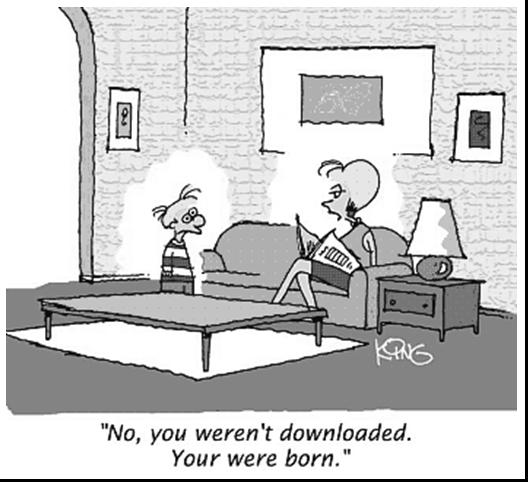
\includegraphics[width=.5\textwidth]{fig1.jpg}
\caption{A typical figure}
\label{fig:exampleFig1}
\end{figure}

\begin{figure}[ht]
\centering
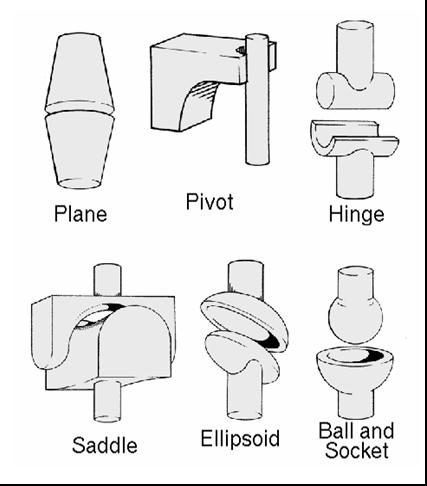
\includegraphics[width=.3\textwidth]{fig2.jpg}
\caption{This figure is an example of a figure caption taking more than one
  line and justified considering margins mentioned in Section~\ref{sec:figs}.}
\label{fig:exampleFig2}
\end{figure}



\begin{table}[ht]
\centering
\caption{Variables to be considered on the evaluation of interaction
  techniques}
\label{tab:exTable1}
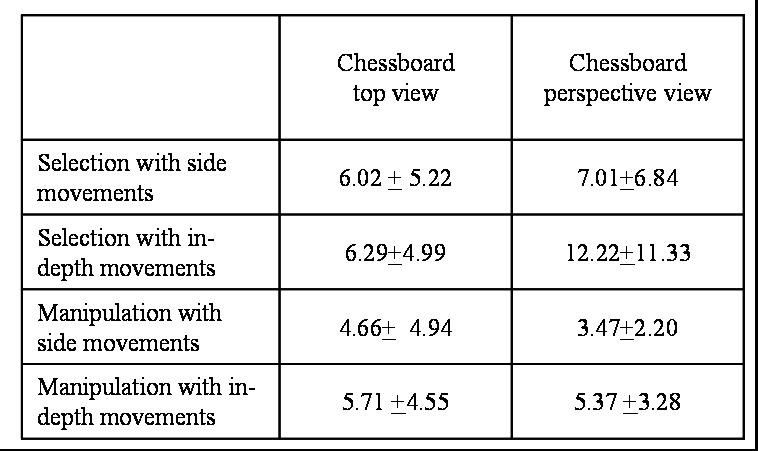
\includegraphics[width=.7\textwidth]{table.jpg}
\end{table}

\section{Images}



\section{References}

Bibliographic references must be unambiguous and uniform.  We recommend giving
the author names references in brackets, e.g. \cite{knuth:84},
\cite{boulic:91}, and \cite{smith:99}.

The references must be listed using 12 point font size, with 6 points of space
before each reference. The first line of each reference should not be
indented, while the subsequent should be indented by 0.5 cm.

\bibliographystyle{sbc}
\bibliography{sbc-template}

\end{document}
